To investigate the influence of layup materials, heat flux variations, vehicle diameter and the trajectory approach on the \gls{tps} a sensitivity analysis is performed. First different materials are selected to form multiple lay-ups. The different lay-ups are then optimised for different loading conditions: the influence of heat flux variations on areal density is investigated. Subsequently, variations in mass due to changing diameters are tested. Lastly, the layups are tested for different trajectories, either with a direct trajectory or with an orbit between aerocapture and landing. This investigation is done by using the tool described in Section \ref{subsec:thermaltool}.

\paragraph{\gls{tps} materials}
Table \ref{tab:tpsmatprop} shows some promising materials that can be used in the inflatable heat shield \cite{Corso2009,Corso2011,DuPont2011,Smith2011}. These materials have been proposed during the design of multiple inflatable decelerator concepts. For each material the thermal conductivity, the density, the specific heat, the maximum operative temperature and if applicable, the emissivity are given. The latter is only applicable to the top  thermal protection layers, because these layers will radiate heat into the surroundings.\\

Using the same reference a selection is made for the most promising thermal protection and insulation layers. These are Nextel BF-20 and Nicalon for the thermal protection layers. For the insulation layers these are Pyrogel 3350 and Pyrogel 6650. With those materials three layups are created whom are validated in Appendix \ref{sec:VandVthermo}. A schematic view of the layers is shown in Figure \ref{fig:layersensthermal}. These layups will be tested for different heat fluxes as well as different diameters.

\begin{table}[ht]
	\caption {flexible \acrfull{tps} material properties}
	\centering
	\begin{tabular}{|l|l|l|l|l|l|l|}
		\hline
		\textbf{Material}         & \textbf{ $\mathbf{k}$ $\mathbf{\left[\frac{W}{m\cdot K}\right]} $} & \textbf{ $\mathbf{ \rho }$ $\mathbf{ \left[ \frac{kg}{m^3} \right] }$} & \textbf{  $\mathbf{ c_{p} }$ $\mathbf{ \left[ \frac{J}{kg \cdot K} \right] }$ }& \textbf{ $\mathbf{ T_{max} }$ $\mathbf{ [ K ] }$} &\textbf{ $\mathbf{ \varepsilon }$ $\mathbf{ [ - ] }$} & \textbf{Function} \\[1.6ex]   \hline \hline
		Viton       & 0.202 & 1842 & 1654 & N/A	 & 0.85 & rad. coating
		\\ \hline
		Nextel AF14       & 0.150                                                 & 858                                        & 1050                                            & 1373	 & 0.443    & rad. \& barrier                                 \\ \hline
		Nextel BF20       & 0.146 
		& 1362                                        & 1130 
		& 1643	 & 0.443  & rad. \& barrier                                  
		\\ \hline
		Nextel XN513      & 0.148                                                 & 1151                                       & 1090                                            & 1673	 & 0.443           & rad. \& barrier                               \\ \hline
		Refrasil C1554-48 & 0.865                                                 & 924                                        & 1172                                            & 1533	 & 0.7     & rad. \& barrier                                       \\ \hline
		Refrasil UC100-28 & 0.865                                                 & 890                                        & 1172                                            & 1255  & 0.2       & rad. \& barrier                                    \\ \hline
		Hexcel 282 Carbon & 0.5                                                   & 891                                        & 1000                                            & N/A 	 & 0.9      & rad. \& barrier \\ \hline
		Pyrogel 6650      & 0.030                                                 & 110                                        & 1046                                            & 923    & ~        & insulator                                  \\ \hline
		Pyrogel 5401      & 0.0248                                                & 170                                        & 1046                                            & N/A  	 & ~          & insulator                                 \\ \hline
		Refrasil 1800      & 0.085                                                 & 156                                        & 1172                                            & 1255 	 & ~           & insulator                                \\ \hline
		Refrasil 2000      & 0.095                                                 & 180                                        & 1172                                            & 1366 	 & ~            & insulator                               \\ \hline
		KFA 5             & 0.25                                                  & 98                                         & 1250                                            & 1473 	 & ~        & insulator                                   \\ \hline
		Nomex             & 0.035                                                  & 384                                         & 1465                                            & N/A 	 & ~        & insulator                                   \\ \hline
		Kapton            & 0.12                                                  & 1468                                       & 1022                                            & 673	 & ~            & gas barrier                              \\ \hline
		Upilex            & 0.29                                                  & 1470                                       & 1130                                            & 773 	 & ~             & structural                            \\ \hline
		Kevlar            & 0.04 & 1440                                       & 1420                                            & 443 	 & ~             & structural                            \\ \hline
		Vectran            & 0.37 & 1400 & 1259 & N/A 	 &  & structural                            \\ \hline
	\end{tabular}
	\label{tab:tpsmatprop}
\end{table}

\begin{figure}[h]
	\centering
	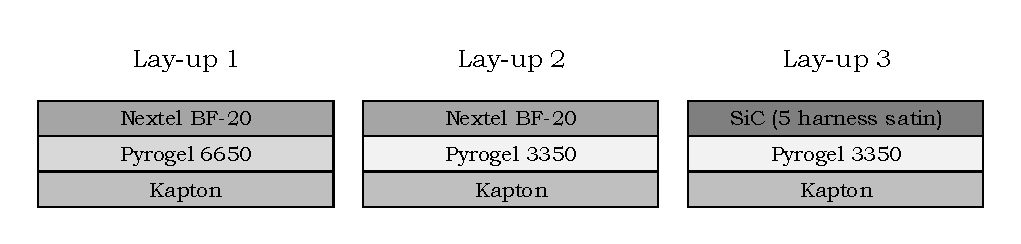
\includegraphics{./Figure/Thermal/layersensthermal.pdf}
	\caption{Tested lay-ups for the sensitivity analysis}
	\label{fig:layersensthermal}
\end{figure}

\paragraph{Effect of heat flux}

In order to analyse layup mass performance and changes due to variable atmospheric conditions a heat flux sensitivity is performed. The heat flux of a possible trajectory is multiplied by scaling factors to find relative values. The trajectory is found using a diameter of 12 $ \left[ m \right]$ and the relative factors are 0.25, 0.5, 0.75, 0.9, 1.0, 1.1, 1.4, 1.5, 2.0, 2.5 and 3.0. The results are shown in Figure \ref{fig:sensiticvityq}. The horizontal axis show the relative factors and the areal density is shown on the vertical axis. 

\begin{figure}[h]
	\centering
	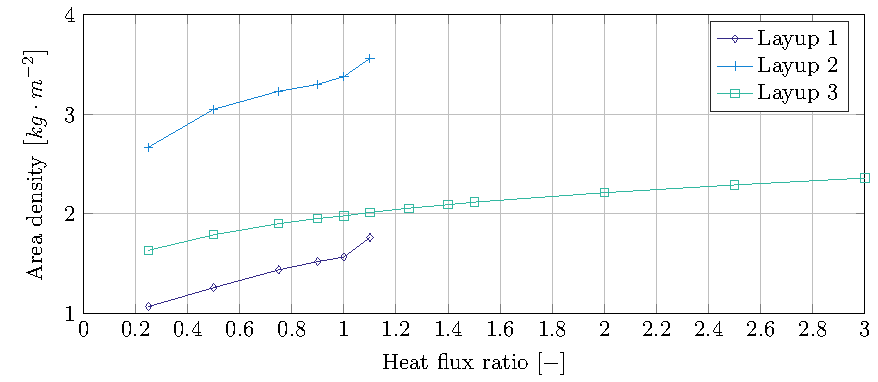
\includegraphics{./Figure/Thermal/Sensitivityq.pdf}
	\caption{heatflux sensitivity for the three selected layups}
	\label{fig:sensitivityq}
\end{figure}


As expected, the mass of the \gls{tps} increases with increasing loading. Secondly and most important, the relative performance of the layups can be observed. layup 1 is clearly the lightest solution, followed by layup 3 and 2. However, although layup 1 performs better in terms of its mass, the amount of loading it can bear is limited. If small changes in atmospheric properties occur during the \gls{edl} phase, for instance due to Martian storms, the \gls{tps} may succumb under the increasing loads. Therefore it is wise to choose Nicalon for further design. Lastly, if layup 1 and 3 are analysed relative to each other, it is clear that Pyrogel 6650 performs much better than the 3350 variant. Therefore, for further design it is more favourable to use Pyrogel 6650 as an insulator.

\paragraph{Effect of diameter}
The three lay-ups are put to the test for different diameters. Aerodynamic analysis has provided heat fluxes for trajectories for shapes with corresponding diameters of 6, 9, 12, 15 and 18 $\left[ m \right]$. As a side note, because the aerodynamic shape is different from the one in the previous paragraph, Figures \ref{fig:sensitivityq} and \ref{fig:sensitivityA} cannot be compared 1:1. An increase in heat flux caused an increase in the maximum temperature, surpassing the Nextel operative temperature limit which made it impossible for layups 1 and 3 to fly trajectories at diameters of 12 $\left[ m \right]$. Optimising the thickness of the lay-ups for these heat flux result in Figure \ref(fig:sensitivityA). the solid lines indicate the nominal trajectory, with orbit after aerocapture. For both graphs, the horizontal axis shows the relevant diameters. On the vertical axis the left figure shows the areal density and the right plot shows the total mass of the frontal \gls{tps}. 

\begin{figure}[h]
	\centering
	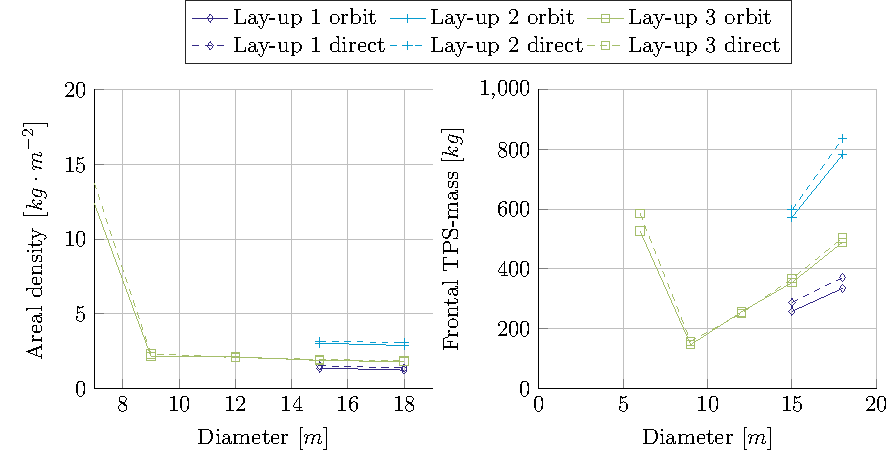
\includegraphics{./Figure/Thermal/SensitivityA.pdf}
	\caption{Areal sensitivity for the three selected layups, both for a direct trajectory and a usual trajectory with orbit after aerocapture. Left pot shows areal mass, whereas the right plot shows the total mass.}
	\label{fig:sensitivityA}
\end{figure}

For increasing diameters, larger radii of curvature can be obtained, resulting in a direct decrease of incomming heat flux. Also, due to the increasing diameters which causes an increase in \gls{sym:CD} and a reduction in ballistic coefficient, the vehicle can decelerate by the same amount at lower dynamic pressures. Therefore, the vehicle can stay higher in the atmosphere and fly in thinner air with the same velocity, decreasing heat development and incoming heat flux.\\

This effect can clearly be seen in the left figure, where the areal density decreases for increasing diameters. Obviously more material must be used to create larger \gls{tps}, which mostly results in a total mass increase for larger diameters. This can be seen in the right figure. The only exception is layup 2, the layup that is able to coop with the larger incoming heat flux at lower diameters. An optimum of its thermal performance is found at 9 $ \left[ m \right] $ where the frontal \gls{tps}-mass reduces to approximately 150 $ \left[ kg \right] $. In addition, the relative mass performance of the different layups is comparable to the performance in the previous paragraph.

\paragraph{Effect of time}
Whenever the vehicle is changing its descend rate, the total dissipated energy is still the same. However, the energy rate profile will have a different distribution over time, changing the temperature throughout the \gls{tps}. Steeper descends require a thicker heat barrier, limiting the heat flow to the rest of the shell, such that operational temperature of the insulator is not exceeded. A more gradual descend increases the time spend in the atmosphere and therefore increases the heat stored in the heat shield. This puts limits on the insulators minimum thickness, to block the heat flow to the structural layers and the rest of the vehicle. Therefore, the effect of descent time is analysed. The results are also shown in Figure \ref{fig:sensitivityA}. An alteration in time is visible by considering two types of viable trajectories, a direct trajectory and one with an orbit after aerocapture. From the figure it can be seen that the direct trajectory is the limiting one. \\
